\documentclass[../main.tex]{subfiles}	

\begin{document}

\chapter{Domain Adaptation}
\label{ch:domain_adaptation}

In the last chapter of this thesis work, we want to address another important field of machine learning, with which we can complete our previous discussion about condition monitoring, i.e. domain adaptation. Domain adaptation is an area of \textit{transfer learning}, dedicated to the study of those scenarios in which we aim at generalizing an high performance learner on a target domain via utilizing the knowledge distilled on a source domain which has a different but related data distribution.\\
The starting point of this last analysis is the observation that those simulations, constructed to collect the data we have used to approach the healthy-faulty classification problems in the last chapter, have some inherent dissimilarities with the real-world situations. We expect, in fact, to have much less faulty conditions in practice, and so the datasets we have used up to now were not properly balanced, with fault signals being overrepresented. This is the main reason for which we need a working strategy suitable to extend, to \textit{transfer}, the knowledge that our models learned from simulated data to a "target" set, constituted by more "realistic", often unlabeled, samples. And this strategy can be found exactly in this area known as domain adaptation. \\
In particular, we are going to deepen a recent transfer learning strategy known as \textbf{Wasserstein Distance Guided Representation Learning} (WDGRL) \cite{shen2018wasserstein}, that we believe it could be the starting point for future studies in domain adaptation for complex-valued deep learning. This approach is, in fact, based on the optimization problem of a measure that can we can extend, without ambiguity, also in the complex domain, i.e. the Wasserstein Distance. \\
We also made several tests considering a possible alternative to WDGRL, also this with a trivial extent in the complex domain, i.e. \textbf{Adversarial Domain Adaptation} \cite{adversarial_domain_adaptation, ajakan2015domainadversarial, ganin2016domainadversarial}.
We didn't manage, however, to obtain any consistent and/or stable result using this methodology, and so we decided only to cite it.\\
We believe that the nice results (at least qualitatively) we have achieved, could be a nice starting point for future, more detailed works, as apparently, no domain adaptation approach has been proposed for complex-valued inputs yet.

\section{Wasserstein Distance Guided Representation Learning}

One of the most common strategies for domain adaptation is to learn domain-invariant feature representations that have to be also discriminative in prediction. To do this, usually domain adaptation frameworks are based on both a learning approach to measure and reduce the domain discrepancy, as well as a discriminator for classification.\\
The method we are going to present now, in particular, has been inspired by Generative Adversarial Networks: in GANs, in fact, there are two adversarial networks playing a \textit{minimax} game in which the discriminator is trained to distinguish real
data the artificial ones, while the generator learns to produce high-quality samples to fool its opponent.\\ 
It is intuitive to employ this minimax game for domain adaptation to make the source and target feature representations indistinguishable. The main problem of this strategy is that, if we setup a second "domain classifier" with the the objective of distinguishing among source and target samples (like in DANNs), we will likely face vanishing gradients. The innovative idea, here, is to replace the domain discrepancy measure with a \textit{Wasserstein Distance}, which provides more stable gradients, even if the two distributions are distant \cite{shen2018wasserstein}. Essentially, the strategy proposed consists into training a "critic" network to estimate the empirical Wasserstein distance between the source and the target features representation, projected into an high level latent space thanks to a "feature extractor". This last network, will then be optimized in order to minimize the estimated metric in an adversarial manner, with the purpose of learning a feature representation that is invariant with respect to the covariate shift between domains.\\
The innovation brought by this method is the introduction of this Wasserstein Distance in the field of domain adaptation. This metric quantifies the distance among two distributions (source and target), $\mathds{P}_s$ and $\mathds{P}_t$, as follow:
\[ W_1(\mathds{P}_s, \mathds{P}_t) = \sup_{\norm{f}_L\leq 1} \mathds{E}_{x\sim\mathds{P}_s}\left[f(x)\right] - \mathds{E}_{x\sim\mathds{P}_t}\left[f(x)\right] \]
where the Lipschitz semi-norm is defined as $\norm{f}_L = \sup\abs{f(x)-f(y)}/d(x,y)$. We noticed that all those mathematical quantities (expectation values, norm and distance) can be extended without ambiguity also in the complex plane, and so we adopted this method in our complex-valued deep learning framework.\\
So, looking at the practical implementation, we will need to setup three independent architectures (a \textit{Feature Extractor}, a \textit{Discriminator} and a \textit{Critic}, like in figure \ref{fig:wdgrl_scheme}) each one with its own training parameters, and loss function to optimize:
\begin{itemize}
	\item for the discriminator, we simply have to minimize the crossentropy among predictions and true labels of source data:
	\[ \mathscr{L}_c(x^s, y^s) = \frac{1}{n_s}\sum_{i=1}^{n^s}\sum_{k=1}^{l}\mathds{1}(y_i^s=k) \cdot\log f_c(f_g(x_i^s))_k \]
	where $f_c$ and $f_g$ are the functions learned by the classifier and the feature extractor, respectively;
	\item for the critic, we have to solve the problem
	\[ \max_{\theta_w}\left\{\mathscr{L}_{wd} - \gamma\mathscr{L}_{grad}\right\}  \qquad\text{with}\qquad \mathscr{L}_{wd}(x_s) = \frac{1}{n_s}\sum_{x^s\in X^s}f_w(f_g(x^s)) -  \frac{1}{n_t}\sum_{x^t\in X^t}f_w(f_g(x^t)) \]
	where $\mathscr{L}_{wd}(x_s)$ is the domain critic loss, i.e. the Wasserstein distance among source and target samples, $\mathscr{L}_{grad}$ is a penalty term introduced to avoid exploding gradients, $\theta_w$ are the parameters of the critic network (with respect to which we have to maximize that difference) and $\gamma$ is a balancing term;
	\item for the feature extractor, instead, the loss function is simply the difference of the first two:
	\[ \mathscr{L}_{g} = \mathscr{L}_{c} + \lambda\mathscr{L}_{wd}  \]
	with $\lambda$ quantifying the trade-off among the two contributes.
\end{itemize}
In the end, the optimization we are performing is an adversarial training characterized by the \textit{minimax} problem:
\[ \min_{\theta_g,\theta_c}\left\{\mathscr{L}_{c}+\lambda\max_{\theta_w}\left[\mathscr{L}_{wd}-\gamma\mathscr{L}_{grad}\right]\right\} \]


\begin{figure}[!ht]
	\centering
	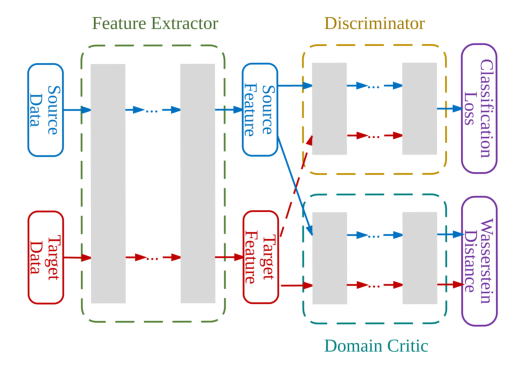
\includegraphics[width=0.7\textwidth]{pictures/wdgrl_scheme}
	\caption{Network scheme of Wassersten Distance Guided Representation Learning applied to a classification task.}
	\label{fig:wdgrl_scheme}
\end{figure}



\section{Domain Adaptation of Bonfiglioli Data}

In section \ref{sec:mendeley_analysis}, with the objective of showing the generalization properties of complex-valued models, we divided the Mendeley dataset into smaller subsets, according to their specific time-varying speed conditions, and we trained the model over only  some of those. In that case we were able to guarantee nice accuracies in almost all the combinations of training-test sets, proving that dynamical conditions do not affect much those high-level features that our models learn from them.\\
The fact is that, in the above case, the experimental setup, except for the rotational dynamics, were identical among train and test subsets. But for the data provided by Bonfiglioli, the situation is much more complicated: those datasets differ not only by the fault simulated, but also by the engine that is begin tested. We will see that both real and complex-valued models underperform, sometimes becoming even completely unable, to distinguish among signals originated by different motors.\\
In order to properly simulate a real-world situation, in which engine's faults are quite rare and most of the signals measured are healthy, we proceeded as follow:
\begin{itemize}
	\item the trials in the source were split into a $75\%-25\%$ train-test sets;
	\item for the trials in the target, the faulty samples were all put in the target-test set, while the healthy samples were split among target-train and target-test sets, with the same percentage as before; in this way the target-train set is completely constituted by healthy samples (even if, officially, from the point of view of the models, those samples are unlabeled). 
\end{itemize}
There are two cases, among the Bonfiglioli datasets, that we found interesting to consider for domain adaptation:
\begin{itemize}
	\item \textit{Trials 4 and 5 versus trial 6}: in this configuration, the source set contains both the information about the mechanical engine (trial 4) and about the kind of fault (trial 5) of the target distribution (trial 6) and so we believe it constitutes the ideal case for testing domain adaptation.
	\item \textit{Trial 10\_1 vs trial 10\_4}: this is a particular case, since the both datasets have been collected over the same setup, with the same rotational gearmotor and same kind of fault; the only difference, in this case, is that the two experimental axis, healthy and faulty, have been inverted (this was done in order to ensure that our machine learning models were not trained to "learn the axis" but to recognize the fault).
\end{itemize}
In both cases, in fact, the classifiers developed, even guaranteeing nice performances over the source distributions, were not able alone to generalize properly over signals belonging to the target distribution, regardless of the similarity of the two.\\
There were also cases in which, even implementing domain adaptation, we weren't able to make the model converge, sign that probably the two distributions are inherently too different among each other. This is the case of \textit{trial 5 vs trial 11}: the two datasets share the same kind of fault simulated, but contains signals collected from different engines, and apparently this constituted an impassable obstacle to generalization (also with conventional real-valued approaches).\\
Regarding the models that we have used in our analysis, we can say that they have essentially the same structure of the ones built in the classification tasks (figure \ref{fig:bonfiglioli_architectures}). The feature extractor is constituted by the first part of the complex-valued model (basically the three convolutional layers) up to the flattening step, while the discriminator and the domain critic are simple multi-layer perceptrons with structure $Linear(32)\to Linear(8)\to Linear(n)$, with $n$ being the number of classes for the first, and $n=1$ for the latter.
 
\subsection*{Trials 4 and 5 versus trial 6}

In this first attempt we consider, as source set, the union of trials 4 (BN90, unbalance) and 5 (BMD118, bearing) while trial 6 (BN90, bearing) will be our target set, split into target-train and target-test as explained above. Let's start showing how limited are the generalization performances of our complex-valued architecture and its real counterpart. For simplicity, we first considered the problem as a binary classification task, with only labels "healthy" and "faulty", and not caring about the two different types of fault. Then, training the networks over the source-train set, we obtain, after the convergence, the accuracy values reported in table \ref{tab:bonfiglioli_binary_generalization_456}.
\begin{table}[!ht]
	\centering
	\begin{tabular}{c | c}
		\toprule
		\textbf{Source-test} & \textbf{Target average}\\
		\midrule
		99.94\% - 99.94\% & 65.28\% - 59.59\% \\
		\bottomrule
	\end{tabular}
\caption{Generalization accuracies of models in \ref{fig:bonfiglioli_architectures} in the binary domain adaptation problem 4-5 vs 6 (real-complex). The convolutional networks has been trained over the source-train set (trials 4-5) and, after the convergence, evaluated over the remaining three subsets (source-test, target-train and target-test).}
\label{tab:bonfiglioli_binary_generalization_456}
\end{table}
This time we see the real-valued model providing the higher accuracy: we noticed, however, that in the training loop, the crossentropy decreased a lot, much more than in the complex case. Looking also at the results achieved in previous chapters, this could be just a sign of higher overfitting and instability.\\
Running our complex-valued WDGRL algorithm using this input combination, we see the losses effectively converging in figure \ref{fig:wdgrl_results_456_binary}, certifying the functionality of this extent. Furthermore, we see the target-test accuracy fluctuating around high values ($85\%-90\%$), while in table \ref{tab:bonfiglioli_binary_generalization_456}, containing the performances reached without domain adaptation, we stopped at $65\%$.\\
This is a very nice result, proving that complex-valued domain adaptation works and can drastically increase the generalization capabilities of our models. To be honest, however, we noticed that those training loops were characterized by high instability, and we had to make numerous trials before finding combinations of hyperparameters allowing to achieve such good results. For this reason, we believe further studies should be addressed to this, also to reduce the overfitting. Unluckily, we didn't have time, and computational resources, to explore more combinations and alternatives, but we can still be quite satisfied of the results achieved, at least qualitatively, especially because this is an almost unexplored branch of complex-valued deep learning.
\begin{figure}[!ht]
	\centering
	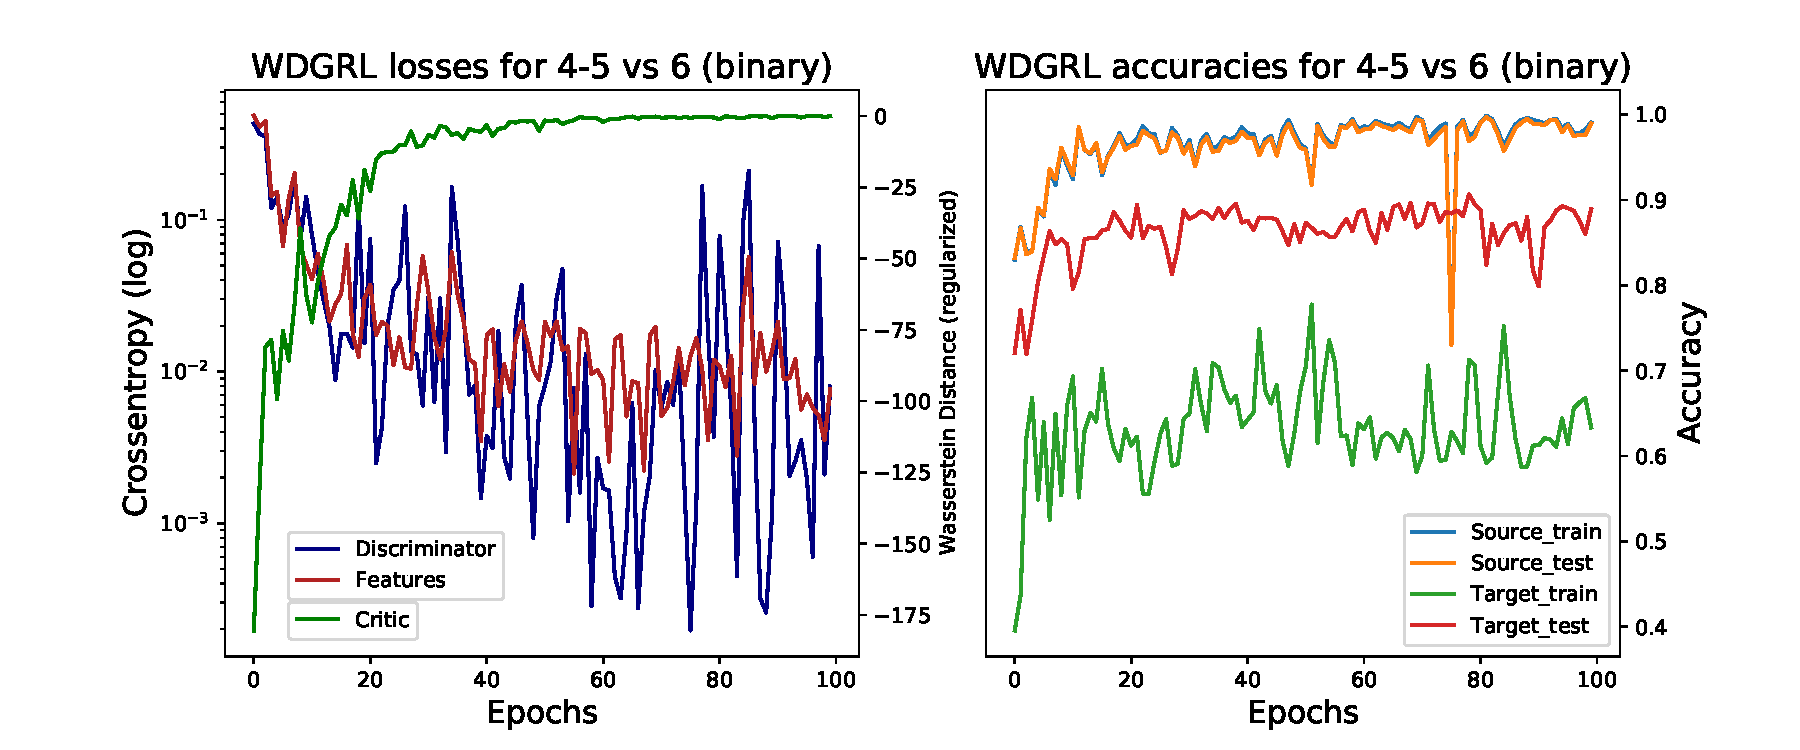
\includegraphics[width=\textwidth]{pictures/wdgrl_results_456_binary}
	\caption{WDGRL training results for the datasets 4-5 vs 6.}
	\label{fig:wdgrl_results_456_binary}
\end{figure}
To simplify the work of domain adaptation, in the test just realized we consider a binary classification problem: what if we keep the two faults (unbalance, for trial 4, and bearing, for trials 5 and 6) distinct? In table \ref{tab:bonfiglioli_multiclass_generalization_456}, we put the results obtained without transfer learning, in the same way as before, but this time with 3 classes to distinguish among.
\begin{table}[!ht]
	\centering
	\begin{tabular}{c | c}
		\toprule
		\textbf{Source-test} & \textbf{Target average}\\
		\midrule
		99.94\% - 99.84\% & 31.28\% - 35.16\% \\
		\bottomrule
	\end{tabular}
	\caption{Generalization accuracies of models in \ref{fig:bonfiglioli_architectures} in the multiclass domain adaptation problem 4-5 vs 6 (real-complex). The convolutional networks has been trained over the source-train set (trials 4-5) and, after the convergence, evaluated over the remaining three subsets (source-test, target-train and target-test).}
	\label{tab:bonfiglioli_multiclass_generalization_456}
\end{table}
The absolute performances decreases drastically, but this time, it is the complex network that wins the competition.\\
We run, also in this case, the complex-valued WDGRL algorithm, and again we get a huge improvement in the final accuracy (over the target-test set): from the $35\%$ (reported in table \ref{tab:bonfiglioli_multiclass_generalization_456}) up to $>60\%$. The instability in this case is higher but the model have also much bigger margin of refinement, starting from such bad performances.


\subsection*{Trial 10\_1 vs trial 10\_4}

We have already presented the peculiarity of this combination of datasets, characterized by the same mechanical components, but with the faults simulated in different axis. Apparently, this is enough to change completely the nature of the signals measured. Repeating the same preliminary tests as for the other configuration (table \ref{tab:bonfiglioli_generalization_101_104}), this time the accuracy values are higher, and we notice a clear advantage of the complex model ($+10\%$).
\begin{table}[!ht]
	\centering
	\begin{tabular}{c | c}
		\toprule
		\textbf{Source-test} & \textbf{Target average}\\
		\midrule
		100.00\% - 99.64\% & 66.46\% - 76.13\% \\
		\bottomrule
	\end{tabular}
	\caption{Generalization accuracies of models in \ref{fig:bonfiglioli_architectures} in the multiclass domain adaptation problem 10\_1 vs 10\_4 (real-complex). The convolutional networks has been trained over the source-train set (trial 10\_1) and, after the convergence, evaluated over the remaining three subsets (source-test, target-train and target-test).}
	\label{tab:bonfiglioli_generalization_101_104}
\end{table}
\begin{figure}[!hb]
	\centering
	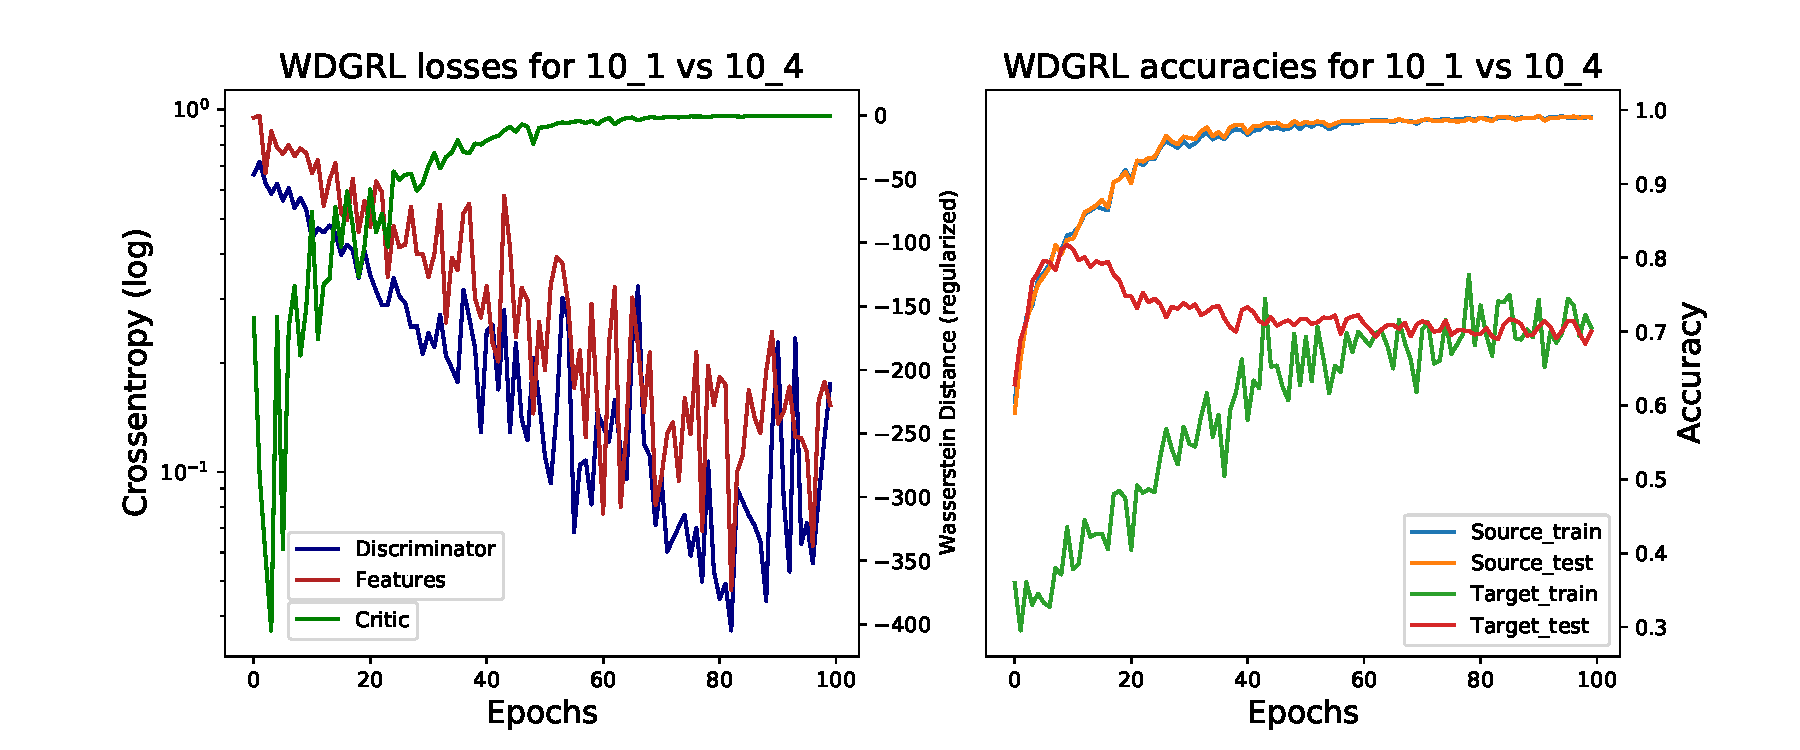
\includegraphics[width=\textwidth]{pictures/wdgrl_results_10}
	\caption{WDGRL training results for the datasets $10\_1$ vs $10\_4$.}
	\label{fig:wdgrl_results_10}
\end{figure}
Differently from before, after running the complex-WDGRL algorithm, we didn't effectively managed to improve the accuracies obtained with the raw networks. The training loop converged, as we can see in figure \ref{fig:wdgrl_results_10}, but we final accuracy was fluctuating always around the $75\%$. We decided to add this plot anyway because it is interesting to observe target-train and target-test accuracies converging to the same value. And the reason is probably that in this case the source and target are more homogeneous internally, at least respect to the other combination of trials.




\end{document}